\documentclass{article}
\usepackage{amsmath}
\usepackage[latin1,utf8]{inputenc}
\usepackage{tikz}
\usetikzlibrary{arrows}
\usetikzlibrary{arrows.meta}
\usetikzlibrary{positioning, shapes.arrows, backgrounds}
\usepackage{xcolor}

\newcommand{\deletionElement}{\alpha}

\begin{document}

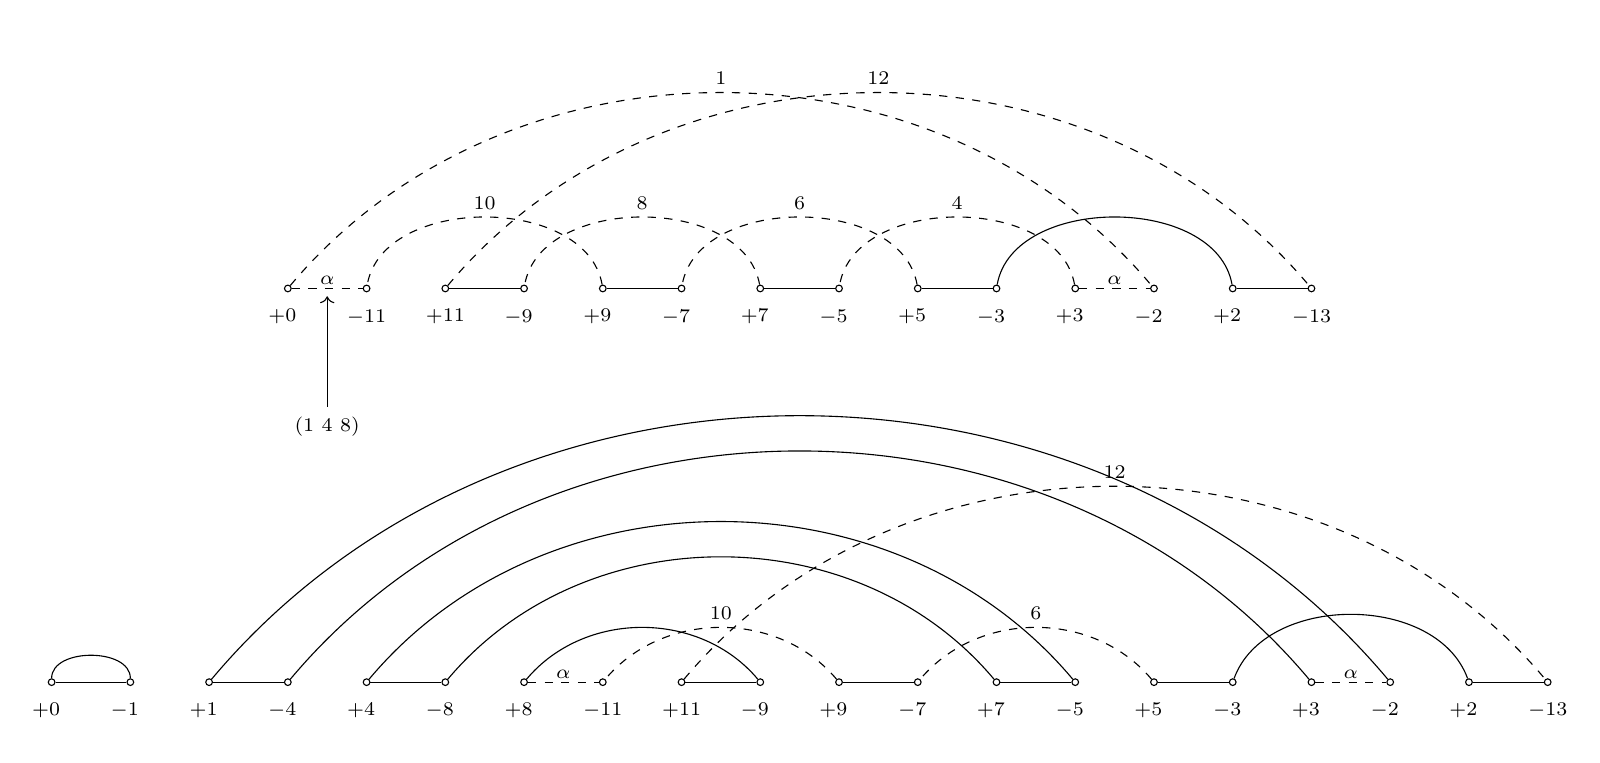
\begin{tikzpicture}[scale=1]
\scriptsize
\begin{scope}[every node/.style={inner sep=0.3mm, draw, circle, minimum size = 0pt}]
    \node[label=below:$+0$\phantom{1}] (p0) at (0,0) {};
    \node[label=below:$-11$] (m6) at (1,0) {};
    \node[label=below:$+11$] (p6) at (2,0) {};
    \node[label=below:$-9$\phantom{1}] (m5) at (3,0) {};
    \node[label=below:$+9$\phantom{1}] (p5) at (4,0) {};
    \node[label=below:$-7$\phantom{1}] (m4) at (5,0) {};
    \node[label=below:$+7$\phantom{1}] (p4) at (6,0) {};
    \node[label=below:$-5$\phantom{1}] (m3) at (7,0) {};
    \node[label=below:$+5$\phantom{1}] (p3) at (8,0) {};
    \node[label=below:$-3$\phantom{1}] (m2) at (9,0) {};
    \node[label=below:$+3$\phantom{1}] (p2) at (10,0) {};
    \node[label=below:$-2$\phantom{1}] (m1) at (11,0) {};
    \node[label=below:$+2$\phantom{1}] (p1) at (12,0) {};
    \node[label=below:$-13$] (m8) at (13,0) {};
\end{scope}

\begin{scope}[every edge/.style={draw=black}]
    \path [<-] (0.5, -0.1) edge (0.5, -1.5);
    \node[] (insertion) at (0.5, -1.75) {(1~4~8)};
\end{scope}

\begin{scope}[every edge/.style={draw=black}]
    \path [-] (p5) edge node [black, pos=0.5, sloped, above] {} (m4);
    \path [-] (p3) edge node [black, pos=0.5, sloped, above] {} (m2);
    \path [-] (p1) edge node [black, pos=0.5, sloped, above] {} (m8);
    \path [-] (p4) edge node [black, pos=0.5, sloped, above] {} (m3);
    \path [-] (p6) edge node [black, pos=0.5, sloped, above] {} (m5);
\end{scope}

\begin{scope}[dashed]
    \path [-] (p0) edge node [black, pos=0.5, sloped, above, yshift=-0.05cm] {$\deletionElement$} (m6);
    \path [-] (p2) edge node [black, pos=0.5, sloped, above, yshift=-0.05cm] {$\deletionElement$} (m1);
\end{scope}

\begin{scope}[every edge/.style={draw=black}]
    \path [-] (p1) edge  [bend right=80] (m2);
\end{scope}

\begin{scope}[dashed]
    \path [-] (p5) edge  [bend right=80] node [black, pos=0.5, sloped, above] {$10$} (m6);
    \path [-] (p0) edge  [bend left=50] node [black, pos=0.5, sloped, above] {$1$} (m1);
    \path [-] (p2) edge  [bend right=80] node [black, pos=0.5, sloped, above] {$4$} (m3);
    \path [-] (p4) edge  [bend right=80] node [black, pos=0.5, sloped, above] {$8$} (m5);
    \path [-] (p3) edge  [bend right=80] node [black, pos=0.5, sloped, above] {$6$} (m4);
    \path [-] (p6) edge  [bend left=50] node [black, pos=0.5, sloped, above] {$12$} (m8);
\end{scope}

\begin{scope}[every node/.style={inner sep=0.3mm, draw, circle, minimum size = 0pt}]
    \node[label=below:$+0$\phantom{1}] (2p0) at (-3,-5) {};
    \node[label=below:$-1$\phantom{1}] (2m1) at (-2,-5) {};
    \node[label=below:$+1$\phantom{1}] (2p1) at (-1,-5) {};
    \node[label=below:$-4$\phantom{1}] (2m4) at (0,-5) {};
    \node[label=below:$+4$\phantom{1}] (2p4) at (1,-5) {};
    \node[label=below:$-8$\phantom{1}] (2m8) at (2,-5) {};
    \node[label=below:$+8$\phantom{1}] (2p8) at (3,-5) {};
    \node[label=below:$-11$] (2m11) at (4,-5) {};
    \node[label=below:$+11$] (2p11) at (5,-5) {};
    \node[label=below:$-9$\phantom{1}] (2m9) at (6,-5) {};
    \node[label=below:$+9$\phantom{1}] (2p9) at (7,-5) {};
    \node[label=below:$-7$\phantom{1}] (2m7) at (8,-5) {};
    \node[label=below:$+7$\phantom{1}] (2p7) at (9,-5) {};
    \node[label=below:$-5$\phantom{1}] (2m5) at (10,-5) {};
    \node[label=below:$+5$\phantom{1}] (2p5) at (11,-5) {};
    \node[label=below:$-3$\phantom{1}] (2m3) at (12,-5) {};
    \node[label=below:$+3$\phantom{1}] (2p3) at (13,-5) {};
    \node[label=below:$-2$\phantom{1}] (2m2) at (14,-5) {};
    \node[label=below:$+2$\phantom{1}] (2p2) at (15,-5) {};
    \node[label=below:$-13$] (2m13) at (16,-5) {};
\end{scope}

\begin{scope}[every edge/.style={draw=black}]
    \path [-] (2p1) edge node [black, pos=0.5, sloped, above] {} (2m4);
    \path [-] (2p4) edge node [black, pos=0.5, sloped, above] {} (2m8);
    \path [-] (2p9) edge node [black, pos=0.5, sloped, above] {} (2m7);
    \path [-] (2p7) edge node [black, pos=0.5, sloped, above] {} (2m5);
    \path [-] (2p5) edge node [black, pos=0.5, sloped, above] {} (2m3);
    \path [-] (2p2) edge node [black, pos=0.5, sloped, above] {} (2m13);
    \path [-] (2p0) edge node [black, pos=0.5, sloped, above] {} (2m1);
    \path [-] (2p11) edge node [black, pos=0.5, sloped, above] {} (2m9);
\end{scope}

\begin{scope}[dashed]
  
  \path [-] (2p3) edge node [black, pos=0.5, sloped, above, yshift=-0.05cm] {$\deletionElement$} (2m2);
  \path [-] (2p8) edge node [black, pos=0.5, sloped, above, yshift=-0.05cm] {$\deletionElement$} (2m11);

\end{scope}


\begin{scope}[every edge/.style={draw=black}]
    \path [-] (2p0) edge  [bend left=90] (2m1);
    \path [-] (2p1) edge  [bend left=50] (2m2);
    \path [-] (2p2) edge  [bend right=70] (2m3);
    \path [-] (2p3) edge  [bend right=50] (2m4);
    \path [-] (2p4) edge  [bend left=50] (2m5);
    \path [-] (2p7) edge  [bend right=50] (2m8);
    \path [-] (2p8) edge  [bend left=50] (2m9);
\end{scope}

\begin{scope}[dashed]
    \path [-] (2p5) edge  [bend right=50] node [black, pos=0.5, sloped, above] {$6$} (2m7);
    \path [-] (2p9) edge  [bend right=50] node [black, pos=0.5, sloped, above] {$10$} (2m11);
    \path [-] (2p11) edge  [bend left=50] node [black, pos=0.5, sloped, above] {$12$} (2m13);
\end{scope}
\end{tikzpicture}

\end{document}